\chapter{\sysname DESIGN}
\label{sec.design}
Our goal is to build a secure network testbed that can mitigate the problem 
of end user's security and privacy issues. 

The previous works introduced in \S{\ref{ssec.related_work}} serves the purpose of understanding the features of current network testbeds. Our finding in \S{\ref{sec.relatedwork_motivation}} suggest that it is important to balance the trade-off between security and functionality.

In this section, we use this idea to guild our new design for building secure network testbed. Our goal is to allow researchers to run experiments while reducing the risk of security and privacy problem.

\section{Overview}
Today's poor visibility into the home networks hampers progress in a number of important research areas, from WiFi management strategies to broadband characterization. Previous works~\cite{sanchez2014measurement}~\cite{dhawan2012fathom} usually provides a programmable interface for writing and launching measurements from the perspective of end systems. Our proposed approach in supporting a wide range of measurements is using a programmable interface as well. Unlike such prior network measurement efforts, our work places network measurement capabilities embedded into home gateway. This approach has various unique advantages: (i) our platform is able to observe all traffic to and from its clients without missing any network traffic. (ii) home gateway is ``demarcation point'' between the home wireless network and the access link so that it is the best place to learn about wired and wireless network. Although BISmark~\cite{183951} has been worked on deploying measurements through the long-term deployment of gateways in homes, it has several security issues that might cripple a user's Internet connection (e.g., malicious codes might run out of router's resource). \sysname instead allows untrusted parties to run any experiment codes on our platform via a programmable interface and resource protection framework. An user can let a third party have access to their network traffic data within a security and performance isolated virtual machine. Users not only are able to control how much information they would share with the rest of world, but also decide how many resources an application can use. For example, an experiment could be prevented when consuming so much resources or access specific interfaces which are not allowed by device's owner. 

\sysname is composed of three separate roles: home wireless router, \sysname provider and experimenter. Router owner donates computational resources to our platform, \sysname provider enables experimenter to pool and share resources, experimenter is seeking to run experiments on remote router.

Before conducting any network measurement experiments, device owner first downloads installer package from \sysname provider which is a testbed server that keep track of routers and allow researcher to access available routers. To run experiment code on owner's router, experimenter needs to download an experiment manager to his own laptop. Experimenter uses the experiment manager to access the remote router directly, upload experiment codes and start or stop the execution of the experiment. Figure~\ref{fig-arch} overviews the different components and their interactions of \sysname.

\begin{figure}%[h]
\centering
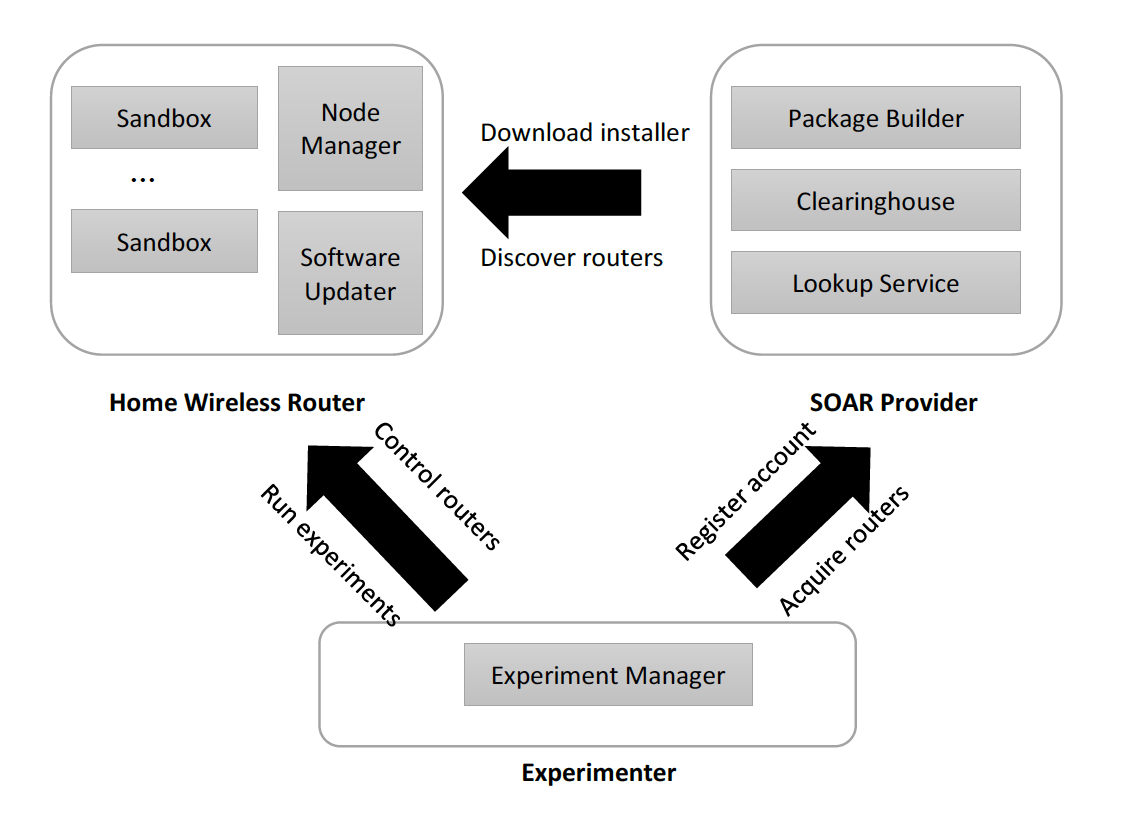
\includegraphics[width=0.8\columnwidth]{figure/soar-arch.png}
\caption{\sysname architecture and different components.}
\label{fig-arch}
\end{figure}

\section{Platform Architecture}
The components in \sysname have three possible roles: the home wireless router (where an experiment runs), the platform provider (that distributes an installer with experimenter's credentials inside) and the experiment manager (where experiments are initiated).

\subsection{Home Wireless Router}
Home wireless routers provide computing resources for experimenters to use in their network measurements. To isolate experiment code from home wireless router, experiment code executes in a \textbf{sandbox} environment. The default sandbox in \sysname is a \sandboxname, a subset of the Linux Kernel API constructed with the Restricted Python sandbox. When experimenters want to deploy their code on a remote router, they need a way to upload code into a sandbox and start it. The \textbf{node manager} listens for remote commands and mediates access to the sandboxes to ensure that only authorize experimenters can execute code in them. Finally, the \textbf{software updater} handles software updates. Once installed, any updates are pushed to nodes automatically instead of searching for new releases of the software manually.  

\subsection{Platform Provider}
The platform provider helps experimenters to pool and share platform resources. A experimenter can distribute a \sysname installer with his credentials inside and share it with router owners. To join \sysname, a router owner first acquire a \sysname installer. The sandbox, nodemanager, software updater and a set of public keys are packaged into this installer by a \textbf{package builder}. After an installation, experimenter uses the public keys to register this node in a \textbf{lookup service} so that this node will be discovered by experimenters.

\subsection{Experiment Manager}
Experimenters use their local machines to initiate and control experiments on a router running \sysname. The \textbf{experiment manager} allows experimenters deploy code into the sandbox and debug the result on router running \sysname. The experiment manager first looks up the set of routers running \sysname associated with an experimenter via the lookup service and then communicates with these nodes, executing commands on the behalf of the experimenter.  

\section{API Design}
{\raggedright
\sysname is a network measurement platform designed to facilitate a broad range of experiments on home gateway while controlling the impact on hosts' resources and network connectivity. A key challenge is selecting a programming interface that is both flexible (i.e., supports a rich set of network measurements) and safe (i.e., does not disrupt a normal user's Internet connectivity). Previous work on sandboxed, programming measurement environments \sysname could server as a useful environment for running network experiments. Considering our goal of supporting a wide range of network measurements on home wireless router, we opt for extending a few capabilities to Repy sandbox\cite{cappos2010retaining}. The Repy sandbox was used to isolate code for the Seattle testbed. The major goals of the sandbox are to provide security and performance isolation, and a portable programming interface across diverse device types. Currently this programming interface provides functions for networking, file system access, threading, locking, logging, and so on. These cover a broad range of network and file I/O capabilities. Repy is highly portable, and has been running in many network measurement projects, such as Content Distribution Network (CDN) Measurements~\cite{rafetseder2011exploring}, Video Streaming and Overlay Routing~\cite{eisl2011service}, Open3GMap~\cite{open3gmap} and so on. Tables \ref{table:new_api} and \ref{table:Repy} provide a summary of our proposed API calls and the current set of measurement capabilities Repy supported. 

Network measurement platforms in today's home networks should support both active and passive measurement. Active measurements require injecting test packets into the network. Traditionally, active measurement tools such as Ping\cite{ping} and Traceroute\cite{traceroute} were used to determine round-trip delays and network topologies. In comparison to the active measurement, the passive measurements do not inject test packets into the network. They need to capture packets and their corresponding timestamps transmitted by the platform. It can provide the information such as availability, utilization, packet errors and discards\cite{calyamactive}. We now briefly describe these capabilities corresponding to network measurements and detailed information about supported network measurements will be mentioned in \S{\ref{sec.network_measurement}}.

\textbf{Basic Statistics.} \texttt{get\_network\_bytes}, \texttt{get\_network\_packets} and \texttt{get\_network\_interface} records aggregate network statistics for passively collected data. These methods read directly and parse data from \emph{/proc/net/dev}. These are able to leverage the naturally-generated network traffic as passive measurements (particularly in the area of broadband characterization) by continuously monitoring the home gateway Internet connection.

\textbf{Wireless Information.} \texttt{scan}, \texttt{get\_station} and \texttt{wifi\_status} provide a python interface to low-level system calls on system. The function sanitizes the call arguments, parsing complex output and return results to the caller. These methods use the \emph{iw} command-line tool to trigger a new WiFi scan and to retrieve its results. \emph{iw} is a new nl80211 based CLI configuration utility for wireless devices. It supports all new drivers that have been added to the kernel recently\cite{iw}. They enable experimenter to study dense WiFi networks and home networks characteristics.

\textbf{Measurement Tool.} \texttt{ping} and \texttt{traceroute} serves as the basis for active measurements. These tools can be combined to build a wide range of measurements experiments. They also are able to contribute to local network debugging. In order to let these measurement tools support on diverse operating systems, we use pure raw socket method to implement it. 


\begin{table*}
\scriptsize
\centering
\begin{tabular}{|p{.2\textwidth}| p{.4\textwidth}| m{.6\textwidth}|}
\hline
\textbf{API}    &  \textbf{Description} \\
 \hline
 {\bf scan} & {\bf Collect the list of access points found with a WiFi scan. For each access point we collect BSSID, SSID, signal strength and channel number.} \\
\hline
 {\bf get\_station} & {\bf Record downlink statistics per associated client (e.g., Total packets sent, received, retried, client's signal strength in home wireless router).} \\
\hline
 {\bf wifi\_status} & {\bf Collect a list of WiFi channel information. (e.g., frequency, channel busy time, channel active time, channel receive time and channel transmit time).} \\
\hline
 {\bf get\_network\_interface} & {\bf Return a list of available network interfaces.} \\
\hline
 {\bf get\_network\_bytes} & {\bf Record information about the configured network interfaces. The statistics include metrics such total number of received or transmitted bytes, drops, errors.} \\
\hline
 {\bf get\_network\_packets} & {\bf Record information about the configured network interfaces. The statistics include metrics such total number of received or transmitted packets, drops, errors.} \\
\hline
 {\bf ping} & {\bf A pure python ping implementation using raw sockets.} \\
\hline
 {\bf traceroute} & {\bf Return the route packets take to network host. } \\
\hline
\end{tabular}
\caption {A summary of our proposed API calls.}
\label{table:new_api}
\end{table*}

\begin{table*}[]
\centering
\begin{tabular}{|l|l|lll}
\cline{1-2}
Network                                                                                                                                                                                                                                                                                         & File system                                                                                                                                         &  &  &  \\ \cline{1-2}
\begin{tabular}[c]{@{}l@{}}gethostbyname\\ getmyip\\ sendmessage\\ openconnection\\ socket.close\\ socket.send\\ socket.recv\\ listenforconnection\\ tcpserversocket.getconnection\\ tcpserversocket.close\\ listenformessage\\ udpserversocket.getmessage\\ udpserversocket.close\end{tabular} & \begin{tabular}[c]{@{}l@{}}openfile\\ close\\ readat\\ writeat\\ listfiles\\ removefile\end{tabular}                                                &  &  &  \\ \cline{1-2}
Threading                                                                                                                                                                                                                                                                                       & Miscellaneous                                                                                                                                       &  &  &  \\ \cline{1-2}
\begin{tabular}[c]{@{}l@{}}createlock\\ lock.acquire\\ lock.release\\ createthread\\ sleep\\ getthreadname\end{tabular}                                                                                                                                                                         & \begin{tabular}[c]{@{}l@{}}log\\ getruntime\\ randombytes\\ exitall\\ createvirtualnamespace\\ getresources\\ virtualnamespace.evalute\end{tabular} &  &  &  \\ \cline{1-2}
\end{tabular}
\caption{Current set of measurement capabilities Repy supported}
\label{table:Repy}
\end{table*}

\begin{table*} 
\scriptsize
\centering
\begin{tabular}{|p{.1\textwidth}| p{.3\textwidth}| m{.3\textwidth}|}
\hline
\textbf{Type} & \textbf{Parameters} & \textbf{Descriptions} \\
 \hline
 {\bf Passive} & {\bf Aggregate traffic statistics per associated client (e.g., Total packets sent, received, retried,
client\'s signal strength at AP)\newline neighbor APs information \newline Channel utilization} & {\bf Home network usage patterns\newline Wireless network performance} \\
\hline
 {\bf Active} & {\bf Throughput, Latency, Loss, Jitter \newline traceroute \newline DNS lookups} & {\bf ISP performance \newline Large-scale topology mapping} \\
\hline
\end{tabular}
\caption {Network measurements obtained from \sysname}
\label{table:experiment}
\end{table*}

\section{Supported Network Measurements.}
\label{sec.network_measurement}
We begin by presenting examples of measurement efforts that benefit from the platform location (at the hub of home networks) and supported capabilities. The list here is far from exhaustive; our design is general, and hence adaptable to a range of other experiments as well. Table~\ref{table:experiment} shows network measurements obtained from \sysname.

\begin{itemize}
\item \textbf{Wireless network performance:} Unlike prior wireless measurement studies that have deployed passive monitors\cite{mahajan2006analyzing}\cite{raghavendra2009wi}\cite{papagiannaki2006experimental}, in our work we take a different approach: We collect wireless performance metrics using these home wireless routers as vantage points. Currently, \sysname supports to gather a variety of wireless network metrics, such as signal strength, tx/rx bitrate, SSID, BSSID, channel number, channel busy time.  Unlike out-of-band wireless monitors, our wireless access points can exactly observe all traffic to and from its clients, correlate them with wireless performance, and hence conduct multiple types of measurements. In addition, home router sits between the access link and wireless network so that it is better to identify and isolation problems between these two locations.

\item \textbf{ISP performance:} The home wireless router is ideally suited for measuring access link characteristics without being affected by confounding factors from the rest of home network. A wide range of network I/O primitives we supported can perform active measurement from home routers to a server, including speed test, performance diagnostics and so on. For example, downloading small binary files through TCP connection from a web server to router to estimate the connection speed.

\item \textbf{Large-scale topology mapping:} Many prior works from research community have tried to understand the Internet's topology and connectivity by conducting \texttt{traceroute-like} measurements from multiple vantage points.\cite{paxson1996end}\cite{chen2009sidewalk} A router-based platform that support \texttt{traceroute} functinality would help researchers to extend their study.

\item \textbf{Home network usage patterns:} Since our platform sits between the access link and the rest of the home network and acts as a continuous monitoring software, we can study home network usage pattern, such as the amount of traffic and the number of devices on the network at any given time. For instance, \texttt{get\_station} is able to gather information about the number of connected devices and \texttt{get\_network\_bytes} have the ability to know the amount of network traffic.    
\end{itemize} 
\par}
\section{Security}
\label{sec.security}
With the rapid development of smart home, it becomes essential to focus on home network security and privacy. Since \sysname deploys on the home wireless router, any bugs may bring a significant impact to home networks. For instance, attackers may obtain the control authority of the home networks through a malicious attack. 

To understand how to prevent attacks, we first considered the different kinds of attacks. A sample of known network attacks is listed in Table~\ref{table: attack}. We observe that these attacks fall into three types: (i) Denial-service attack: overwhelm targets with a flood of network traffic to run out of end host resources, (ii) Injection attack: create a few ``magic'' packets to implement spoof attack or exploit attack. (iii) Insider attack: malicious insiders intentionally eavesdrop, steal, or damage information to violate user's privacy.

\begin{table*}[]
\centering
\begin{tabular}{|l|l|l}
\cline{1-2}
Classes of attack     & Example                                 &  \\ \cline{1-2}
Denial-service attack & Packet flooding, SYN flooding\cite{eddy2011syn}             &  \\ \cline{1-2}
Injection attack      & Remote exploits\cite{shellcode},  spoofing attack\cite{bishop1996attack} &  \\ \cline{1-2}
Insider attack        & Network eavesdropping                   &  \\ \cline{1-2}
\end{tabular}
\caption{Common known attacks in networks.}
\label{table: attack}
\end{table*}

To prevent these three types of attacks, \sysname uses a sandboxes environment named Repy for security isolation and performance isolation. 
\begin{itemize} 
\item \textbf{Security isolation:} The sandbox must be able to ensure the execution safety of experiment code while representing as little risk to host as possible. The Repy sandbox in \sysname uses language-based isolation and is implemented in Python. In addition, Repy uses security layer to push library functionality out of the sandbox kernel, thereby helping to mitigate the impact of bugs in libraries~\cite{cappos2010retaining}. As a result, experimenter can enforce a policy upon a Repy sandbox without needing to change the TCB (trusted computing base).  
\item \textbf{Performance isolation:} Resource consumption is the biggest issue for a distributed system. Especially when we are in the home networks and need to share our platform with unidentified home wireless routers. The rate of resource consumption may degrade the performance of itself and others in real network when vulnerabilities comes into effect\cite{joshi2013survey}. Therefore, \sysname must control the load its experiments impose on the routers, as well as minimize the impact of real user's network connectivity. To achieve it, \sysname should limit consumption of host's resources, include the amount of CPU and memory used, network and disk I/O. To control CPU and memory utilization, \sysname monitors the amount of CPU and memory available to a experiment. To control network and disk I/O, \sysname checks calls that access these resources and prevents their execution if they exceed a predefined limits. 
\end{itemize}

Through performance isolation, the volume of experiment's network traffic is restricted based on the quota router owner predefined. Therefore, denial-service attack is impossible because our platform does not allow to launch a sustained flood of traffic to other hosts. In addition, since sandbox control CPU, memory, bandwodth, disk I/O and other resources, \sysname is able to control the load of its experiments impose on the local host. Through security isolation, experimenter has the ability of setting up policy for library and returned data. For instance, if one wants to restrict access to certain functionality's parameter or returned value, this can be added in a secure policy without changing Repy. To mitigate the second and third types of attacks, we could block few functionalities that may pose risks to home networks and anonymize sensitive information that will leverage users' privacy, the detail information will be discussed in \S{\ref{sec.privacy}}. 

\section{Privacy}
\label{sec.privacy}
Although a rich set of capabilities enhance the convenience of user interfaces and application usefulness, they also raise serious privacy concerns. For example, network traffic volume over interface and the information of connected devices in home networks produce a rich history, it will lead to behaviour prediction, such information invades user privacy. 

In order not to allow measurements to exfiltrate sensitive information from home gateway, \sysname provides a framework of reference monitor~\cite{ref}, to enforce mandatory access control to sensitive data in real time. Firgure~\ref{fig-reference} shows the overview of reference monitor. Different from modifying the sandbox, \sysname allows users to decide not only what information experimenters can capture on their routers, but also how much information they would share with others. \sysname allows router owner to add privacy filters they wish to apply. These may range from sharing home network devices information with experimenter by blocking MAC addresses or completely denying access to network traffic statistics. For a particular experiment, a privacy policy might based on the type of network measurement, the capabilities can be passed through, filtered, or dropped by the reference monitor. For example, an experimenter who wants to learn about Internet censorship, a filter might perform an action such as removing access point information from WiFi scans and network traffic volume information in home networks, only allow to access ping and traceroute functionality. These privacy filters are easily built and disseminated to router owners. Therefore, \sysname is able to handle the second and third types of attacks in Table~\ref{table: attack}. 

\begin{figure}%[h]
\centering
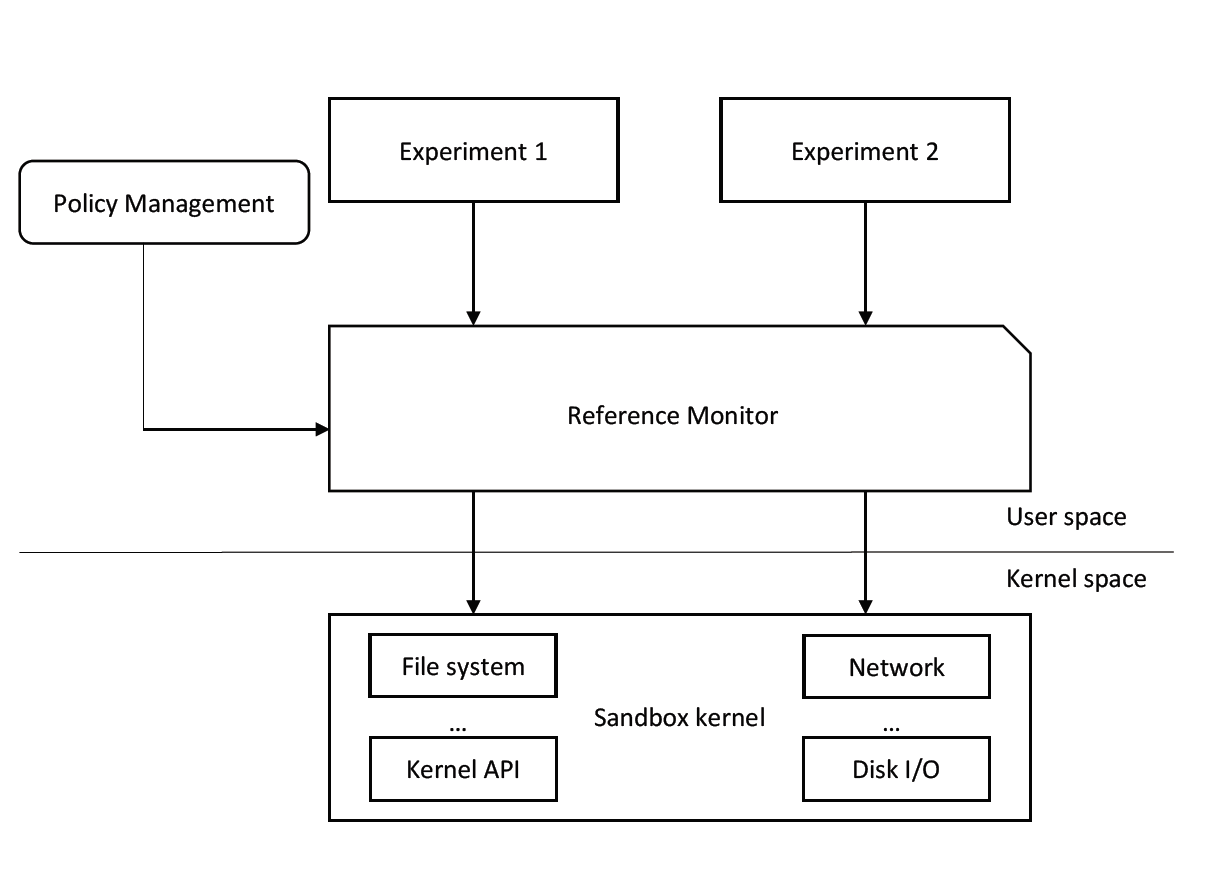
\includegraphics[width=0.8\columnwidth]{figure/referencemonitor.png}
\caption{Overview of reference monitor. The original Repy interface and the added API together provide the OS level sandbox kernel on a home wireless router. Before an experiment can access data, different policies can be combined together as a set of filters to protect users' privacy.}
\label{fig-reference}
\end{figure}

